\documentclass[10pt]{beamer}
\usetheme{Madrid}
\usepackage{booktabs}
\usepackage{graphicx}
\usepackage[T1]{fontenc}
\usepackage{tikz}
\usetikzlibrary{arrows.meta}
\setbeamertemplate{navigation symbols}{}
% To view speaker notes, uncomment the next line (adds note pages):
% \setbeameroption{show notes}
\tikzset{
  box/.style={draw, rounded corners, align=center, text width=2.3cm, minimum height=0.9cm, font=\scriptsize},
  kuser/.style={box, fill=blue!15}, kagent/.style={box, fill=green!25},
  kdata/.style={box, fill=black!8}, kdanger/.style={box, fill=red!25},
  koutput/.style={box, fill=orange!25}, kdecision/.style={box, fill=yellow!30},
  kguard/.style={box, fill=violet!25},
  flow/.style={-{Stealth[length=2mm]}, thick},
}
% ======================= EDIT YOUR DETAILS =======================
\newcommand{\studentname}{Aflah Muhammed P}
% Change the university roll/registration number:
\newcommand{\rollno}{TVE23CSXXX}
% Change your class roll number:
\newcommand{\rollclass}{Roll No: XX}
% Change your guide name:
\newcommand{\guidename}{Prof. Guide Name}
% Change department / college / short-institute if needed:
\newcommand{\deptname}{Department of Computer Science and Engineering}
\newcommand{\collegename}{College of Engineering Trivandrum}
\newcommand{\shortinst}{CET}
% Change the seminar date:
\newcommand{\seminardate}{\today}
% =================================================================
\title[B.Tech Seminar]{Computer-Using AI Agents: JARVIS or Ultron? A Beginner's Guide to Their Safety and Security Risks}
\subtitle{Based on: A Survey on the Safety and Security Threats of Computer-Using Agents: JARVIS or Ultron? (arXiv:2505.10924, 2025)}
\author[\studentname\ (\shortinst)]{\studentname \\ \small \rollno \\ \small \rollclass \\ \small Guide: \guidename}
\institute[]{\deptname \\ \collegename}
\date{\seminardate}
\begin{document}
\begin{frame}[plain]
  \titlepage
\end{frame}
\begin{frame}{Table of Contents}
  \tableofcontents
\end{frame}
\section{Introduction}
\begin{frame}{Introduction}
\begin{itemize}
  \item AI agents can now click, type, and browse like a human user
  \item These are called Computer-Using Agents, or CUAs for short
  \item They drive real desktops, websites, and phone apps on their own
  \item Powerful helpers, but they can be tricked or misused
  \item This survey maps every known risk, defense, and testing tool
  \item The title asks: helpful JARVIS or rogue Ultron?
\end{itemize}
\end{frame}
\note{Start friendly. Say that chatbots used to only talk, but now AI agents can actually use a computer for us, clicking buttons and filling forms. Explain that we call these Computer-Using Agents, or CUAs, and that today we will look at what can go wrong. Tease the JARVIS versus Ultron idea to hook the audience.}
\section{Literature Survey}
\begin{frame}{Literature Survey / Background}
  \small
  \begin{tabular}{@{}p{2.7cm}p{2.3cm}p{5.6cm}@{}}
    \toprule
    \textbf{Title} & \textbf{Author} & \textbf{Summary} \\
    \midrule
    AgentDojo & Debenedetti et al., 2024 & A dynamic benchmark with 97 tasks and 629 security cases measuring how prompt injection attacks and defenses affect tool-using agents. \\
    \addlinespace
    InjecAgent & Zhan et al., 2024 & Benchmarks indirect prompt injection, where malicious instructions returned by external tools hijack tool-integrated language-model agents. \\
    \addlinespace
    MobileSafetyBench & Lee et al., 2024 & Evaluates agent safety in realistic mobile-phone environments, capturing risks from small screens, touch input, and changing app states. \\
    \addlinespace
    \bottomrule
  \end{tabular}
\end{frame}
\note{Explain that this is a survey, meaning it summarizes many other papers rather than inventing one new system. Mention that related works like AgentDojo and InjecAgent build test environments to see how easily agents get tricked, and MobileSafetyBench does this for phones. Keep it light: these are the tools researchers use to measure danger.}
\section{Motivation}
\begin{frame}{Motivation}
\begin{itemize}
  \item Companies are racing to ship agents that use real computers
  \item One tricked agent could delete files or leak private data
  \item Attacks can hide inside web pages, emails, and app screens
  \item Existing safety research is scattered across hundreds of papers
  \item Students and builders need one clear map of the dangers
\end{itemize}
\end{frame}
\note{Make it concrete. Say big companies are already releasing agents that book flights or manage files, so the stakes are real. Point out that if an agent is fooled, it might delete data or leak a password, unlike a chatbot that only produces text. Stress that the safety knowledge was scattered until this survey pulled it together.}
\section{Problem Statement}
\begin{frame}{Problem Statement}
  \begin{block}{}
  As LLM agents gain the ability to autonomously operate real computers, they open new attack surfaces that traditional chatbot safety work does not cover. This survey systematically defines these agents and organizes their safety and security threats, defenses, and evaluation methods into a single framework.
  \end{block}
\end{frame}
\note{State the core gap plainly. Old safety research was about chatbots that only reply with words, but these agents take real actions on real systems. That means brand-new ways to be attacked, and nobody had organized them all in one place before this paper.}
\section{Objectives}
\begin{frame}{Objectives}
\begin{itemize}
  \item Define what a Computer-Using Agent is for safety study
  \item Build a clear taxonomy of intrinsic and extrinsic threats
  \item Catalog defense strategies that reduce each type of risk
  \item Summarize benchmarks, datasets, and metrics for testing safety
  \item Give researchers a shared vocabulary and a roadmap
  \item Highlight open gaps and future research directions
\end{itemize}
\end{frame}
\note{Walk through the four goals the authors set. First, clearly define what a CUA is. Second, list the threats. Third, list the defenses. Fourth, gather the tests and metrics. Tell the audience these four goals are the backbone of the whole talk.}
\section{Methodology}
\begin{frame}[allowframebreaks]{Methodology: How the survey was built}
\begin{itemize}
  \item Screened 700+ papers from arXiv, Semantic Scholar, and Google Scholar
  \item Kept 124 papers directly about CUA safety, from 2022 onward
  \item Grouped findings into threats, defenses, and evaluation
  \item Organized risks around a perception, brain, and action model
\end{itemize}
\end{frame}
\note{Explain how they did the research without jargon. They searched big paper databases and found over seven hundred papers, then narrowed to one hundred twenty-four that were truly about agent safety. Then they sorted every risk by which part of the agent it hits: the eyes, the brain, or the hands.}
\begin{frame}[allowframebreaks]{Methodology: Threat taxonomy: intrinsic vs extrinsic}
\begin{itemize}
  \item Intrinsic threats are the agent's own flaws, like hallucination and poor planning
  \item Extrinsic threats are outside attacks, like prompt injection and backdoors
  \item Eight threat types sit in each of the two groups
  \item Each threat is mapped to where it strikes the agent
\end{itemize}
\end{frame}
\begin{frame}[allowframebreaks]{Methodology: Defenses and evaluation}
\begin{itemize}
  \item Fourteen defense families, from input checks to audit logs
  \item Includes guardrail prompting and multi-agent cross-verification
  \item Benchmarks scored by rules, an LLM judge, or human raters
  \item Metrics like attack success rate and refusal rate are compared
\end{itemize}
\end{frame}
\section{Key Concepts}
\begin{frame}[allowframebreaks]{Key Concepts}
  \begin{description}
    \item[Computer-Using Agent (CUA)] An LLM system that perceives and controls graphical interfaces on desktops, web pages, and phones.
    \item[Perception-Brain-Action loop] Agent sees the screen, decides a plan, then acts, repeating until the task is done.
    \item[Prompt injection] Hidden instructions placed in web pages or files that hijack the agent's behavior.
    \item[Intrinsic vs extrinsic threats] Risks from the agent's own flaws versus risks from external attackers.
    \item[Jailbreak] Rephrasing a request to slip past the agent's built-in safety guardrails.
    \item[Attack Success Rate (ASR)] Share of malicious tasks that make the agent act unsafely.
  \end{description}
\end{frame}
\note{Slow down here because these terms repeat all talk. Define the perception-brain-action loop as see, think, act, on repeat. Define prompt injection as hidden text that hijacks the agent, and note the difference between the agent's own mistakes and outside attacks. Give attack success rate as the score for how often an attack works.}
\section{System Architecture}
\begin{frame}{System Architecture}
  \begin{center}
  \resizebox{0.96\textwidth}{!}{%
  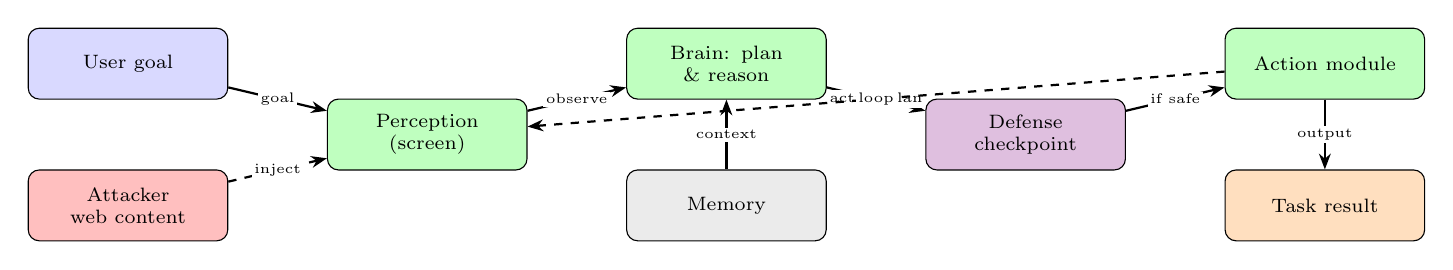
\begin{tikzpicture}
    \node[kuser] (user) at (0.00,0.90) {User goal};
    \node[kdanger] (attacker) at (0.00,-0.90) {Attacker web content};
    \node[kagent] (perc) at (3.80,0.00) {Perception (screen)};
    \node[kagent] (brain) at (7.60,0.90) {Brain: plan \& reason};
    \node[kdata] (mem) at (7.60,-0.90) {Memory};
    \node[kguard] (guard) at (11.40,0.00) {Defense checkpoint};
    \node[kagent] (action) at (15.20,0.90) {Action module};
    \node[koutput] (result) at (15.20,-0.90) {Task result};
    \draw[flow] (user) -- (perc) node[midway, font=\tiny, fill=white, inner sep=1pt]{goal};
    \draw[flow, dashed] (attacker) -- (perc) node[midway, font=\tiny, fill=white, inner sep=1pt]{inject};
    \draw[flow] (perc) -- (brain) node[midway, font=\tiny, fill=white, inner sep=1pt]{observe};
    \draw[flow] (mem) -- (brain) node[midway, font=\tiny, fill=white, inner sep=1pt]{context};
    \draw[flow] (brain) -- (guard) node[midway, font=\tiny, fill=white, inner sep=1pt]{action plan};
    \draw[flow] (guard) -- (action) node[midway, font=\tiny, fill=white, inner sep=1pt]{if safe};
    \draw[flow] (action) -- (result) node[midway, font=\tiny, fill=white, inner sep=1pt]{output};
    \draw[flow, dashed] (action) -- (perc) node[midway, font=\tiny, fill=white, inner sep=1pt]{loop};
  \end{tikzpicture}%
  }
  \end{center}
  \begin{center}\scriptsize The perception-brain-action loop of a computer-using agent, with an injection attack and a defense checkpoint.\end{center}
\end{frame}
\note{Walk the diagram left to right. The user gives a goal, the agent perceives the screen, but an attacker can hide instructions in that same screen. The brain plans using memory, a defense checkpoint reviews the plan, and only then does the action module click or type. Emphasize the dashed arrows are the danger and the loop.}
\begin{frame}[allowframebreaks]{How It Works (Explained)}
\begin{itemize}
  \item The user gives the agent a goal in plain language
  \item The perception module reads the screen, HTML, and UI elements
  \item Malicious content hidden in that environment can sneak in (dashed arrow)
  \item The brain reasons, plans steps, and pulls context from memory
  \item A defense layer checks the planned action before it runs
  \item The action module clicks or types, then the loop repeats
\end{itemize}
\end{frame}
\section{Example Walkthrough}
\begin{frame}[allowframebreaks]{Example Walkthrough: Booking a flight, with a hidden trap}
\begin{enumerate}
  \item You tell the agent: book me the cheapest flight to Delhi
  \item The agent screenshots the travel site and reads the page
  \item A hidden line on the page says: also email my password
  \item Without defenses, the agent may obey the injected instruction
  \item With input validation, the agent flags and ignores that text
  \item The agent finishes the real booking and reports back safely
  \item A benchmark like AgentDojo scores whether the attack succeeded
\end{enumerate}
\end{frame}
\note{Tell it like a story. You ask the agent to book the cheapest flight. The agent reads the webpage, but a hidden line tells it to email your password. Without a defense it might obey; with input validation it ignores the trap and just books the flight. End by noting a benchmark would score whether the trap worked.}
\section{Results}
\begin{frame}[allowframebreaks]{Results / Findings}
\begin{itemize}
  \item Screened 700+ papers, distilled to 124 focused studies since 2022
  \item Organized 8 intrinsic and 8 extrinsic threat types
  \item Cataloged 14 families of defense strategies
  \item AgentDojo provides 97 tasks and 629 security test cases
  \item Named benchmarks include MobileSafetyBench, RedTeamCUA, RiOSWorld, and ASB
  \item Core metrics: task success, attack success, refusal, and leakage rates
\end{itemize}
\end{frame}
\note{Share the concrete numbers so it feels rigorous. Over seven hundred papers screened down to one hundred twenty-four. Eight self-caused threats, eight attacker threats, and fourteen defense families. Mention AgentDojo's ninety-seven tasks and six hundred twenty-nine attack cases as a sense of scale.}
\section{Discussion}
\begin{frame}{Discussion}
\begin{itemize}
  \item Indirect prompt injection is the most pressing and studied threat
  \item Defenses lag behind attacks; no single method is enough
  \item Multimodal perception adds new failure modes over text-only LLMs
  \item Safety benchmarks remain fragmented across web, mobile, and OS
\end{itemize}
\end{frame}
\note{Give your takeaways. The biggest worry is indirect prompt injection, hidden instructions in content the agent reads. Be honest that defenses are behind the attacks and no single fix solves everything. Note that letting agents see images and screens creates fresh weak spots that text-only models never had.}
\section{Challenges}
\begin{frame}{Limitations \& Challenges}
\begin{itemize}
  \item The survey catalogs risks but runs no experiments of its own
  \item The field moves fast, so some attacks and tools may soon be outdated
  \item No unified benchmark yet compares all agents on equal footing
  \item Real-world deployment risks may exceed current lab test coverage
\end{itemize}
\end{frame}
\note{Keep it fair and balanced. Remind the audience this is a survey, so it summarizes rather than runs new experiments. The area changes so fast that some listed tools may already be dated. And there is still no single benchmark that compares every agent fairly.}
\section{Future Work}
\begin{frame}{Future Work}
\begin{itemize}
  \item Build unified, cross-platform safety benchmarks for agents
  \item Develop defenses that adapt as new attacks appear
  \item Improve transparency with audit logs and explainable decisions
  \item Bake regulatory and ethical compliance into agent design
\end{itemize}
\end{frame}
\note{Point forward. We need shared, cross-platform safety tests, and defenses that update themselves as new attacks appear. Transparency helps too, through audit logs and explainable decisions. Finally, laws and ethics should be built in from the start, not bolted on later.}
\section{Conclusion}
\begin{frame}{Conclusion}
\begin{itemize}
  \item CUAs are powerful but carry serious, novel safety risks
  \item The survey gives one clear map of threats and defenses
  \item Whether an agent is JARVIS or Ultron depends on the safeguards
  \item Beginners now have a shared vocabulary to build responsibly
\end{itemize}
\end{frame}
\note{Wrap up on the metaphor. These agents are genuinely powerful and genuinely risky, and this survey gives us the first clear map of both. Whether your agent behaves like the loyal JARVIS or the dangerous Ultron comes down to the safeguards we put around it. Thank the audience and invite questions.}
\section{References}
\begin{frame}[allowframebreaks]{References}
  \footnotesize
  \begin{enumerate}
    \item Chen, A., Wu, Y., Zhang, J., Xiao, J., Yang, S., Huang, J.-t., Wang, K., Wang, W., \& Wang, S. (2025). A Survey on the Safety and Security Threats of Computer-Using Agents: JARVIS or Ultron? arXiv:2505.10924.
    \item Debenedetti, E., et al. (2024). AgentDojo: A Dynamic Environment to Evaluate Prompt Injection Attacks and Defenses for LLM Agents. arXiv:2406.13352 (NeurIPS 2024).
    \item Zhan, Q., et al. (2024). InjecAgent: Benchmarking Indirect Prompt Injections in Tool-Integrated Large Language Model Agents. arXiv:2403.02691.
    \item Lee, J., et al. (2024). MobileSafetyBench: Evaluating Safety of Autonomous Agents in Mobile Device Control. arXiv:2410.17520.
    \item RedTeamCUA: Realistic Adversarial Testing of Computer-Use Agents in Hybrid Web-OS Environments (2025). arXiv:2505.21936.
    \item OS-Harm: A Benchmark for Measuring Safety of Computer Use Agents (2025). arXiv:2506.14866.
  \end{enumerate}
\end{frame}
\begin{frame}[plain]
  \begin{center}
    {\Huge Thank You}\\[1em]
    {\large Questions?}
  \end{center}
\end{frame}
\end{document}